\documentclass{report}
\usepackage[utf8]{inputenc}
\usepackage[T1]{fontenc}
\usepackage[francais]{babel}
\LARGE

%%packages pour le code
\usepackage{listings}
\usepackage{color}
\usepackage{textcomp}
\usepackage{tikz}
\usepackage{tabto}
\usepackage{pgfplots}
\usepackage{pdfpages}
\usepackage{graphicx}
%%

\title{Rapport de Programmation : Reversi}

\author{Louis \bsc{Coumau}}
\date{Novembre 2019}


\begin{document}

\lstset{language=C, numbers=left, numberstyle=\tiny,stepnumber=1,numbersep=5pt, %basicstyle=\scriptsize,
%upquote=true,
%aboveskip={1.5\baselineskip},
%columns=fullflexible,
%showstringspaces=false,
%extendedchars=true,
%breaklines=true,
%showtabs=false,
%showspaces=false,
%showstringspaces=false,
identifierstyle=\ttfamily,
keywordstyle=\color[rgb]{0,0,1},
commentstyle=\color[rgb]{0.133,0.545,0.133},
stringstyle=\color[rgb]{0.627,0.126,0.941},
}

\maketitle %indique la page de garde avec les informations décrites plus haut

\tableofcontents



\chapter{Implementation}

\section{Interface generale}
L'interface est importante, elle va nous permettre d'interagir avec le jeu. Il faut donc qu'elle soit la plus fiable possible, et qu'elle informe sur le conportement de ce de dernier tout en restant simple à comprendre.
\subsection{Norme d'erreur}
La gestion des erreurs et de son affichage se fera dans le fichier reversi.c. elles se présenteront de la facon suivante : \texttt{reversi: t: i} avec

- \texttt{t} le type de l'erreur

- \texttt{i} l'indication concernant l'erreur

Pour certaines des erreurs comme la lecture d'un fichier sans droit, il est renvoyé le numéro de l'erreur concernée.

\subsection{Le mode verbose}
Le mode verbose est le mode permettant de voir le comportement des joueurs et la disposition du plateau tout au long du jeu.
Dès lors que l'option est donnée en argument, une variable booléenne global, initialement définit à faux, devient vrai.
Lorsqu'une simple partie est lancé sans l'option, le jeux affiche les informations suivantes : \newline
\newline
\texttt{Welcome to this reversi game !\newline
Black player (X) is human and white player (O) is human.\newline
Black player start !\newline
\newline
Playing...}\newline

Ensuite, dans le cas où le joueur est humain, le jeux va présenter le plateau et demander un coup.

À la fin de la partie, le plateau final et le score sont affichés : \newline\newline
\texttt{Game over.\newline
\newline
\tabto{1 cm}A B C D E F G H\newline
\tabto{0.62 cm}  1 O O O O O O O O\newline
\tabto{0.62 cm}  2 O O X X O X X X\newline
\tabto{0.62 cm}  3 X O X O X O X O\newline
\tabto{0.62 cm}  4 X X O O O O X O\newline
\tabto{0.62 cm}  5 X X O O O O X O\newline
\tabto{0.62 cm}  6 X O X O O O O O\newline
\tabto{0.62 cm}  7 X X O X X O O O\newline
\tabto{0.62 cm}  8 X O O O O O O O\newline
\newline
Score: 'X' = 22, 'O' = 42\newline
Player 'O' win the game.}\newline

Lorsqu'un joueur aléatoire\footnote{On définira et expliquera un peut plus tard ce type de joueur.} joue, aucun détail sur son action est affiché. Ainsi, si deux joueur aléatoires joue l'un contre l'autre, les seuls informations affichées serons celles du début
de partie et celle de fin de partie. Contrairement au mode verbose qui, à chaque fois qu'un joueur va poser un pion, et ce quelque soit le type de joueur, va préciser quel coup le joueur à joué et dessiner une limitation entre chaque tour.

Par exemple, voici un échantillon d'affichage dans le cas ou l'on fait jouer un joueur aléatoire contre un autre avec l'option verbose :\newline
\texttt{\newline
X player's turn.\newline
\newline
\tabto{1 cm}A B C D E F G H
\tabto{0.62 cm}  1 X * * * * O \_ X \newline
\tabto{0.62 cm}  2 O X O * O O X X \newline
\tabto{0.62 cm}  3 * O X X * O O X \newline
\tabto{0.62 cm}  4 \_ * O X X O O X \newline
\tabto{0.62 cm}  5 X X X O O X * X \newline
\tabto{0.62 cm}  6 \_ X * O O * O X \newline
\tabto{0.62 cm}  7 \_ \_ * * X O * * \newline
\tabto{0.62 cm}  8 \_ \_ \_ \_ * \_ \_ \_ \newline
\newline
Score: 'X' = 19, 'O' = 17\newline
\newline
X plays D2\newline
==========================================\newline
\newline
O player's turn.\newline
\newline
\tabto{1 cm}A B C D E F G H
\tabto{0.62 cm}  1 X * * * * O * X \newline
\tabto{0.62 cm}  2 O X X X X X X X \newline
\tabto{0.62 cm}  3 \_ O X X * O O X \newline
\tabto{0.62 cm}  4 \_ * O X X O O X \newline
\tabto{0.62 cm}  5 X X X O O X * X \newline
\tabto{0.62 cm}  6 * X * O O * O X \newline
\tabto{0.62 cm}  7 \_ \_ \_ * X O \_ \_ \newline
\tabto{0.62 cm}  8 \_ \_ \_ \_ * * \_ \_ \newline
\newline
Score: 'X' = 23, 'O' = 14\newline
\newline
O plays C6\newline
==========================================\newline}

\section{API board.c}
\subsection{Les bitboard}

Les bitboards sont des entiers dont les bits de la valeur binaire représentent l'état d'une case d'un tableau. \'Etant donné que la taille du plateau sur lequel nous jouons varie entre $2\times2$ et $10\times10$, la taille d'un bitboard doit donc être d'au moins 100 bit pour être capable de représenter tout le plateau. Or, un type de valeur doit être une puissance de 2. Ainsi, nos bitboards seront de taille 128 bits.

Avant de commencer à utiliser de tels entiers, nous allons définir la convention suivante : la case 0,0 (la case tout en haut à gauche du plateau) sera représenté par le bit de poids faible.\newline
\newline
Ci- dessous, un exemple de plateau et sa représentation binaire :
\begin{center}

\renewcommand{\arraystretch} {1.5}
    \begin{tabular}{|p{0.2cm}|c|c|c|}
        \hline
        1 & 0 & 1 & 1\\
        \hline
        0 & 0 & 0 & 0 \\
        \hline
        0 & 0 & 0 & 0 \\
        \hline
        0 & 0 & 0 & 0 \\
        \hline
    \end{tabular}

\end{center}
\begin{center}
        \title{plateau de taille $4\times4$}
\end{center}

\begin{center}
\renewcommand{\arraystretch} {1.5}
       \begin{tabular}{|c|c|c|c|c|c|c|c|c|c|c|c|}
        \hline
        ... & 0 & 0 & 0 & 0 & 1 & 1 & 0 & 1 \\
        \hline
    \end{tabular}
\end{center}

Avec cette convention, l'initialisation d'un bitboard en fonction de la taille d'un plateau et de sa position est évidente.


\subsection{Implementation des fonctions shifs}

Les fonctions shifts on pour but de déplacer des pions sur le plateau dans une direction donné. Pour cela, nous allons utiliser l'opérateur\footnote{Pour manipuler les bitboard, il y a plusieurs types d'opération élémentaires : '\&' qui est le 'ET' logique, '|' qui est le 'OU' logique \textit{(On parlera d'ajout)}, '$\sim$' qui est le 'NON' logique et le décalage expliqué ci-après. } bit à bit >> (resp. <<) qui est le décalage des bit vers la droite (resp. gauche).

\subsubsection{shift-north}

Le déplacement vers le nord est de plus simple à implémenter car, comme vu plus haut, le bit de poids faible est en haut à gauche, il suffit donc de décaler les bits vers la droite (du bit de poids fort au bit de poids faible) autant de fois qu'il y a de case dans une ligne.
Par exemple, prenons encore une fois le plateau de taille $4\times4$ :

\begin{center}
\renewcommand{\arraystretch} {1.5}
    \begin{tabular}{|p{0.2cm}|c|c|c|}
        \hline
        1 & 0 & 0 & 0\\
        \hline
        0 & 1 & 0 & 0 \\
        \hline
        0 & 0 & 1 & 0 \\
        \hline
        0 & 0 & 0 & 1 \\
        \hline
    \end{tabular}

\end{center}
\begin{center}
        \title{Disposition initiale du plateau. \textit{On utilisera toujours cette disposition initiale.}}
\end{center}

En y appliquant le shift-north, soit le décalage des bits vers la droite cela donne :

\begin{center}
\renewcommand{\arraystretch} {1.5}
    \begin{tabular}{|p{0.2cm}|c|c|c|}
        \hline
        0 & 1 & 0 & 0\\
        \hline
        0 & 0 & 1 & 0 \\
        \hline
        0 & 0 & 0 & 1 \\
        \hline
        0 & 0 & 0 & 0 \\
        \hline
    \end{tabular}

\end{center}
\begin{center}
        \title{Disposition après un shift-north}
\end{center}

\subsubsection{shift-south}

La fonction shift-south est légèrement plus subtile car, si on décale les bits vers la droite, certains sont toujours présents en dehors du plateau. On va donc devoir utiliser une valeur permettant de retirer tout les bits dépassants du plateau (masque).

\begin{center}
\renewcommand{\arraystretch} {1.5}
    \begin{tabular}{|p{0.2cm}|c|c|c|}
        \hline
        0 & 0 & 0 & 0\\
        \hline
        1 & 0 & 0 & 0 \\
        \hline
        0 & 1 & 0 & 0 \\
        \hline
        0 & 0 & 1 & 0 \\
        \hline
        0 & 0 & 0 & 1 \\
    \end{tabular}

\end{center}
\begin{center}
        \title{Disposition après un shift-south}
\end{center}

\begin{center}
\renewcommand{\arraystretch} {1.5}
    \begin{tabular}{|p{0.2cm}|c|c|c|}
        \hline
        0 & 0 & 0 & 0\\
        \hline
        1 & 0 & 0 & 0 \\
        \hline
        0 & 1 & 0 & 0 \\
        \hline
        0 & 0 & 1 & 0 \\
        \hline
        0 & 0 & 0 & 1 \\
    \end{tabular}
    \& $\sim$
    \begin{tabular}{|p{0.2cm}|c|c|c|}
        \hline
        0 & 0 & 0 & 0\\
        \hline
        0 & 0 & 0 & 0 \\
        \hline
        0 & 0 & 0 & 0 \\
        \hline
        0 & 0 & 0 & 0 \\
        \hline
        1 & 1 & 1 & 1 \\
    \end{tabular}
    =
     \begin{tabular}{|p{0.2cm}|c|c|c|}
        \hline
        0 & 0 & 0 & 0\\
        \hline
        1 & 0 & 0 & 0 \\
        \hline
        0 & 1 & 0 & 0 \\
        \hline
        0 & 0 & 1 & 0 \\
        \hline
        0 & 0 & 0 & 0 \\
    \end{tabular}

\end{center}
\begin{center}
        \title{Calcul d'un shift-south}
\end{center}

\textit{On notera que $a \& \sim b$ permet de 'retirer' les bits de b à a}

\subsubsection{shift-west}

De même que pour shift-south, lorsque l'on va décaler les bits d'un cran vers la droite (vers la gauche sur le plateau) on va devoir utiliser un masque.

\begin{center}
\renewcommand{\arraystretch} {1.5}
    \begin{tabular}{|p{0.2cm}|c|c|c|}
        \hline
        0 & 0 & 0 & 1\\
        \hline
        1 & 0 & 0 & 0 \\
        \hline
        0 & 1 & 0 & 0 \\
        \hline
        0 & 0 & 1 & 0 \\
        \hline
    \end{tabular}
    \& $\sim$
    \begin{tabular}{|p{0.2cm}|c|c|c|}
        \hline
        0 & 0 & 0 & 1\\
        \hline
        0 & 0 & 0 & 1 \\
        \hline
        0 & 0 & 0 & 1 \\
        \hline
        0 & 0 & 0 & 1 \\
        \hline
    \end{tabular}
    =
     \begin{tabular}{|p{0.2cm}|c|c|c|}
        \hline
        0 & 0 & 0 & 0\\
        \hline
        1 & 0 & 0 & 0 \\
        \hline
        0 & 1 & 0 & 0 \\
        \hline
        0 & 0 & 1 & 0 \\
        \hline
    \end{tabular}

\end{center}
\begin{center}
        \title{Calcul d'un shift-west}
\end{center}

\subsubsection{shift-est}

Le fonctionnement de shift-est est quasiment identique à celui de shift-west :

\begin{center}
\renewcommand{\arraystretch} {1.5}
    \begin{tabular}{|p{0.2cm}|c|c|c|}
        \hline
        0 & 1 & 0 & 0\\
        \hline
        0 & 0 & 1 & 0 \\
        \hline
        0 & 0 & 0 & 1 \\
        \hline
        1 & 0 & 0 & 0 \\
        \hline
    \end{tabular}
    \& $\sim$
    \begin{tabular}{|p{0.2cm}|c|c|c|}
        \hline
        1 & 0 & 0 & 0\\
        \hline
        1 & 0 & 0 & 0 \\
        \hline
        1 & 0 & 0 & 0 \\
        \hline
        1 & 0 & 0 & 0 \\
        \hline
    \end{tabular}
    =
     \begin{tabular}{|p{0.2cm}|c|c|c|}
        \hline
        0 & 1 & 0 & 0\\
        \hline
        0 & 0 & 1 & 0 \\
        \hline
        0 & 0 & 0 & 1 \\
        \hline
        0 & 0 & 0 & 0 \\
        \hline
    \end{tabular}

\end{center}
\begin{center}
        \title{Calcul d'un shift-est}
\end{center}

\subsection{La fonction trace}
Lorsque le joueur actuel\footnote{On définit le joueur actuel comme le joueur à qui c'est le tour de jouer. On notera que ce dernier peut ne pas pouvoir jouer.} peut jouer, il pose un de ces pion sur la case correspondante à la position donné par ce joueur. Or, d’après la règle, tout les pions adverses se trouvant entourés à partir du pion précédemment posé se 'retournent'\footnote{On parle de pion qui se retourne lorsque ce dernier change de joueur.}, et cela, quelque soit la direction.
J’ai donc implémenté une fonction permettant de retrouver la 'trace' de tous les pions à retourner à partir du pion posé. Elle renvoie un bitboard qui n’a plus qu’à être retiré (ajouté) du board représentant les pions de l'adversaire (joueur actuel resp.).\newline

L'algorithme est le suivant : \newline

- pour toutes les directions,

\tabto{1 cm}- tant que le pion rencontré est celui de l'adversaire
\tabto{1 cm}- on ajoute ce pion à la trace

- on retourne la trace des pions à retirer

\subsection{L'itérateur de coup à jouer}
Un peu plus tard, lors de l'implémentation des joueur, nous aurons besoin de savoir si le joueur actuel peut jouer un coup, et si oui, lequel.

C'est pourquoi nous allons ecrire la fonction \texttt{board\_next\_move()} qui va nous renvoyer les coups possibles du joueur actuel, au fur et à mesure de son itération.

Tout d'abord, interessons nous au plateau suivant dans lequel les bits sont des coups possibles :

\begin{center}
\renewcommand{\arraystretch} {1.5}
    \begin{tabular}{|p{0.2cm}|c|c|c|}
        \hline
        0 & 0 & 1 & 0\\
        \hline
        0 & 1 & 0 & 0 \\
        \hline
        0 & 0 & 1 & 0 \\
        \hline
        1 & 0 & 0 & 0 \\
        \hline
    \end{tabular}

\end{center}
\begin{center}
        \title{}
\end{center}

On souhaite récupérer le premier coup à jouer en partant de la case 0,0. Comment déterminer la position de ce premier coup ?

Déjà, on voit bien qu'il est simple de récupérer la coordonné de la colonne en utilisant l'opérateur modulo avec le nombre de zéro précédent. Ensuite, on veut que, suivant une action entre la taille du plateau et ce nombre de zéro, on ait 0 comme coordonné de la ligne.

On s'aperçoit que, pour $i$ quelconque, si $i<size$, la valeur entière de $i/size = 0$, de même, si $size$ $\le$ $i<2\times size$, la valeur entière de $i/size = 1$.

Ainsi, nous pouvons déterminer les coordonnées de ce coup avec le nombre de zéro qui le précède.\newline

Comment calculer le nombre de 0 avant le premier bit ?\newline

Nous allons précéder de la manière suivante.

Reprenons le bitboard précédent :
\begin{center}
\renewcommand{\arraystretch} {1.5}
    \begin{tabular}{|p{0.2cm}|c|c|c|c|c|c|c|c|c|c|c|c|}
        \hline
        1 & 0 & 1 & 0 & 0 & 0 & 0 & 1 & 0 & 0 & 1 & 0 & 0\\
        \hline
    \end{tabular}
\end{center}

On retire 1 ce qui donne :
\begin{center}
\renewcommand{\arraystretch} {1.5}
    \begin{tabular}{|p{0.2cm}|c|c|c|c|c|c|c|c|c|c|c|c|}
        \hline
        1 & 0 & 1 & 0 & 0 & 0 & 0 & 1 & 0 & 0 & 0 & 1 & 1\\
        \hline
    \end{tabular}
\end{center}

On applique l'opération suivante :

\begin{center}
\renewcommand{\arraystretch} {1.5}
    \begin{tabular}{|p{0.2cm}|c|c|c|c|c|c|c|c|c|c|c|c|}
        \hline
        1 & 0 & 1 & 0 & 0 & 0 & 0 & 1 & 0 & 0 & 1 & 0 & 0\\
        \hline
    \end{tabular}
\end{center}
\begin{center}
    $\wedge$\footnote{Opérateur du 'OU EXCLUSIF'}
\end{center}
\begin{center}
\renewcommand{\arraystretch} {1.5}
    \begin{tabular}{|p{0.2cm}|c|c|c|c|c|c|c|c|c|c|c|c|}
        \hline
        1 & 0 & 1 & 0 & 0 & 0 & 0 & 1 & 0 & 0 & 0 & 1 & 1\\
        \hline
    \end{tabular}
\end{center}
\begin{center}
    =
\end{center}
\begin{center}
\renewcommand{\arraystretch} {1.5}
    \begin{tabular}{|p{0.2cm}|c|c|c|c|c|c|c|c|c|c|c|c|}
        \hline
        0 & 0 & 0 & 0 & 0 & 0 & 0 & 0 & 0 & 0 & 1 & 1 & 1\\
        \hline
    \end{tabular}
\end{center}

À ce stade, il ne nous reste plus qu'a utiliser la fonction \texttt{popcount()} pour compter le nombre de bits à 1 dans ce bitboard et retirer 1 au résultat.

Ainsi, nous avons comme formule générale : \newline

\texttt{nbr\_tz\footnote{number of trailing zeroes} = bitboard\_popcount((possibles\_moves-1) $\wedge$ possibles\_moves)-1;}\newline

\textit{Il existe la fonction \texttt{\_\_builtin\_ctz()} du compilateur \texttt{gcc} qui fait exactement la meme chose que la formule ci dessus. Cependant, elle n'est pas adapté pour les entiers de 128 bits. De plus, meme si on l'utilise à la place de la formule sur des entiers uniquement de 64 bits, l'execution n'est pas plus rapide.}

\section{Les types de joueurs}
Apres avoir codé les fonctions de \texttt{board.c}, nous avons à présent une API nous permettant de manipuler des plateaux de jeu. Il nous faut donc implémenter les différents types de joueurs.

\subsection{Le joueur aléatoire}
Le joueur aléatoire est le plus simple de tous les joueurs. son objectif est simplement, comme son nom l'indique, de jouer un coup de façon aléatoire.\newline

Pour cela, nous allons nous aider des fonctions \texttt{board\_count\_player\_moves(board)} qui renvoie le nombre de coup que peux jouer le joueur actuel et \texttt{board\_next\_moves(board)} qui est un littérateur renvoyant succesivement un coup possible du plus proche de la case 0,0 au plus proche de la case size-1,size-1.\newline

L'implementation est la suivante :

- La première étape consiste à récupérer le nombre de coup possible dans \texttt{nbr\_poss\_moves} avec la fonction \texttt{board\_count\_player\_moves(board)}.

- On génère un nombre aléatoire \texttt{r} que l'on réduit dans l'intervalle [0,\texttt{nbr\_poss\_moves}-1] avec le modulo.

- On avance littérateur des coups possibles \texttt{r-1} fois grâce à une boucle \texttt{for}

- Et on retourne le \texttt{r}-ieme coup possible.
\newline

La question que l'on se pose à présent est : comment générer ce nombre aléatoire \texttt{r} ?

Nous allons utiliser la fonction \texttt{random()}. Cependant, pour ce faire, il est nécessaire de mettre à jour la grène aléatoire.

Nous allons donc écrire une fonction \texttt{rand\_init()} qui va vérifier grâce à une variable booléenne statique si la fonction a déjà été exécuté. Si oui, elle ne fait rien, sinon, elle met a jour la grène aléatoire avec \texttt{srandom(time(NULL) - getpid())} et met à vrai la variable de vérification.\newline
\newline
\textit{A partir de maintenant, Nous appellerons 'random\_player' le joueur aléatoire.}


\subsection{Le joueur humain}
Le joueur humain est plus complexe car il nécessite une interaction.

L'objectif de cette fonction est de renvoyer un coup donné. Elle doit donc vérifier si la suite de caractère donné est bien une position possible dans le plateau et si cette position est un coup possible.

\paragraph{\texttt{- get\_column() }}
Intéressons nous tout d'abord à la fonction \texttt{get\_column(char current\_char, size\_t size)} qui permet de vérifier si le caractère \texttt{current\_char} est bien compris entre A et J quelque soit la casse et renvoie sa valeur numérique correspondant à ce caractère. Sinon, elle renvoie size. Effectivement les plateaux que nous utilisons peuvent avoir une taille fixé de $2\times2$, $4\times4$, $6\times6$, $8\times8$ et $10\times10$ soit, au maximum, la colonne J.

\begin{center}
\renewcommand{\arraystretch} {1.5}
       \begin{tabular}{|c|c|c|c|c|c|c|c|c|c|}
        \hline
        A & B & C & D & E & F & G & H & I & J \\
        \hline
        0 & 1 & 2 & 3 & 4 & 5 & 6 & 7 & 8 & 9 \\
        \hline
    \end{tabular}
\end{center}

\paragraph{\texttt{- get\_move() }}

Ensuite, la fonction utilisé pour demander et récupérer les caractères est \texttt{move\_t get\_move(size\_t size)}. Elle exécute les étapes suivantes :

On commence par la partie qui récupère la colonne :

- la variable \texttt{char current\_char} prend la valeur \texttt{getchar()} et on définit \texttt{move\_t move}.

- si ce caractère est \texttt{q} la fonction renvoie le coup \texttt{{size+1,size+1}}.

- sinon on récupère la valeur de \texttt{get\_column(current\_char, size)} dans \texttt{move.column} (on notera que, comme vu plus haut, \texttt{move.column = size} si le caractère est incorrecte)
\newline

Vient ensuite la partie permettant de récupérer le ou les caractères définissant la ligne correspond au coup. Effectivement, le coup donné peut varier entre 1 et 10 et peut donc contenir deux caractères

- on définit un tableau \texttt{char char\_number[2]} de taille 2

- on récupère les caractères dans le tableau.

- \texttt{move.row} prend la valeur du tableau convertie en entier.

- \texttt{move.row} prend la valeur \texttt{size} si cette dernière est égale à 0 ou si elle est supérieur à \texttt{size}

- sinon, on décrémente \texttt{move.row} car on souhaite qu'elle soit dans l'intervalle [0,size-1].

Pour résumer, cette fonction renverra les coups \texttt{size,*} et/ou \texttt{*,size} si l'un des caractères ou l'une des positions sont incorrects et \texttt{size+1,size+1} si le caractère rencontré est q.

\paragraph{\texttt{- human\_player() }}
Nous pouvons maintenant nous intéresser à la fonction principale.


Pour permettre la gestion de la répétition d'un coup, nous allons utiliser une boucle while et une variable booléenne \texttt{error\_case} initialisée à vrai. Cette variable redevient vrai dans les cas ou il est nécessaire de redemander le coup, et faux sinon. Ainsi, la boucle s'arrêtera si aucun de ces cas n'est rencontrés.
Cette dernière s'arrêtera aussi si le caractère entré est \texttt{q}.
Car, comme vu plus haut, dans ce cas, la fonction \texttt{get\_move()} renverra \texttt{size+1,size+1}. Il suffit donc de faire une condition sur uniquement d'une des deux composante de la position retournée.

Il est important de préciser que lorsque l'on a plus besoins de lire un caractère avec \texttt{get\_char()}, il est nécessaire de supprimer les valeurs encore stockées dans ce dernier. Pour ce faire, la fonction \texttt{clean\_buffer()} va appeler \texttt{get\_char()} jusqu'à ce que le caractère retourné par celui ci soit le caractère 'new line'\newline

\textit{À partir de maintenant, nous appellerons 'human\_player' le joueur utilisant la fonction human\_player().}


\subsection{Implementation de l'algorithme Mini-Max}
L'un des principaux objectifs de ce projet et de parvenir à créer un type de joueur capable de gagner quelque soit l'adversaire. Pour ce faire, l'une des méthodes évidente est de parcourir toutes les combinaisons de coup possibles afin de déterminer, lequel permet de prendre le dessus sur l'adversaire. Cependant, en supposant que chaque joueur a au moins 2 coups possibles et qu'ils jouent chacun leur tour sur un plateau de taille 8$\times$8, lors du premier parcourt, il y aura $2^{64}$ possibilités de jeux, ce qui est impossible à faire en un temps raisonnable pour l'instant. C'est pourquoi il est nécessaire de fixer une profondeur.

L'algorithme Mini-Max permet, en fonction du joueur pour lequel il joue et pour chaque configuration du jeu, de lui maximiser une heuristique et, à l'opposé, de minimiser cette heuristique pour le jouer adverse.
Nous commencerons avec une heuristique simple qui ne fait que calculer la différence entre le score du joueur et celui de son adversaire.
\newline

Exemple avec un plateau de taille $4\times4$ :
On suppose que le joueur X est minimax en profondeur 1.


\begin{center}
\renewcommand{\arraystretch} {1.5}
    \begin{tabular}{c|c|c|c|c|}
          &A & B & C & D \\
        \hline
        1 & O & O & O & *\\
        \hline
        2 & X & O & O & * \\
        \hline
        3 & O & X & O & * \\
        \hline
        4 & * & X &  &  \\
        \hline
    \end{tabular}

\end{center}
\begin{center}
    \label{Figure 1}
    \title{Joueur actuel : X ; Scores : X : 3 , O : 7}
\end{center}


C'est au joueur X de jouer. L'algorithme minimax va donc maximiser l'heuristique des 4 coups possibles.

\begin{figure}[!h]
\begin{center}
\renewcommand{\arraystretch} {1.5}
    \begin{tabular}{c|c|c|c|c|}
          &A & B & C & D \\
        \hline
        1 & O & O & O & X\\
        \hline
        2 & X & O & X &  \\
        \hline
        3 & O & X & O &  \\
        \hline
        4 &  & X &  &  \\
        \hline
    \end{tabular}

\end{center}
\begin{center}
    \title{Coup D1}
    \label{Figure 1}
    \caption{Joueur actuel : O ; Scores : X : 5 , O : 6}
    \textit{Dans cette configuration, l'heuristique renvoyé est $5-6=-1$}
\end{center}
\end{figure}

\begin{figure}[!h]
\begin{center}
\renewcommand{\arraystretch} {1.5}
    \begin{tabular}{c|c|c|c|c|}
          &A & B & C & D \\
        \hline
        1 & O & O & O & \\
        \hline
        2 & X & X & X & X \\
        \hline
        3 & O & X & X &  \\
        \hline
        4 &  & X &  &  \\
        \hline
    \end{tabular}

\end{center}
\begin{center}
    \title{Coup D2}
    \label{Figure 1}
    \caption{Joueur actuel : O ; Scores : X : 7 , O : 4}
    \textit{Dans cette configuration, l'heuristique renvoyé est $7-4=3$}
\end{center}
\end{figure}

\begin{figure}[!h]
\begin{center}
\renewcommand{\arraystretch} {1.5}
    \begin{tabular}{c|c|c|c|c|}
          &A & B & C & D \\
        \hline
        1 & O & O & O & \\
        \hline
        2 & X & O & O &  \\
        \hline
        3 & O & X & X & X \\
        \hline
        4 &  & X &  &  \\
        \hline
    \end{tabular}

\end{center}
\begin{center}
    \title{Coup D3}
    \label{Figure 1}
    \caption{Joueur actuel : O ; Scores : X : 5 , O : 6}
    \textit{Dans cette configuration, l'heuristique renvoyé est $5-6=-1$}
\end{center}
\end{figure}

\begin{figure}[!h]
\begin{center}
\renewcommand{\arraystretch} {1.5}
    \begin{tabular}{c|c|c|c|c|}
          &A & B & C & D \\
        \hline
        1 & O & O & O & \\
        \hline
        2 & X & O & O &  \\
        \hline
        3 & X & X & O &  \\
        \hline
        4 & X & X &  &  \\
        \hline
    \end{tabular}

\end{center}
\begin{center}
    \title{Coup A4}
    \label{Figure 1}
    \caption{Joueur actuel : O ; Scores : X : 5 , O : 6}
    \textit{Dans cette configuration, l'heuristique renvoyé est $5-6=-1$}
\end{center}
\end{figure}

Parmis les 4 coups possible, la différence de score du coup D2 est supérieur à celle de tous les autres. Ainsi, le coup renvoyé par minimax à une profondeur 1 sur cette disposition de plateau est D3.

\subsubsection{\texttt{minimax\_machine()}}

Commençons à présent par implementer cette fonction. D'abord, intéressons nous à la fonction \texttt{static int minimax\_machine(board\_t *board, size\_t depth, disc\_t player)} qui prend en paramètre les variables :

- \texttt{board} qui est la structure contenant le plateau sur lequel on joue,

- \texttt{depth} qui est la profondeur d'observation,

- \texttt{player} qui est le joueur pour lequel on veut maximiser l'heuristique.

On va commencer par récupérer le joueur actuel. Ensuite, on continue si ce dernier n'est pas \texttt{EMPTY\_DISC} (cas ou la partie est terminée) et si la profondeur n'est pas égale à 0. Si tel est le cas, on retourne l'heuristique.
\\A ce niveau, 2 cas se présentes \newline

- \underline{Premier cas :}
C'est le cas ou le joueur actuel du plateau est le même que celui pour lequel on souhaite maximiser l'heuristique.
On définit une variable \texttt{best\_score} à \texttt{-INFINITY} \footnote{On notera que, l'on fixe \texttt{INFINITY} à la borne maximal d'un integer, soir $2^{15}-1 = 32767 $.} car on souhaite trouver le maximum parmi plusieurs valeur. Il faut donc que la première valeur de référence soit très petite afin de la remplacer dès la première comparaison.
A ce stade, pour tout les coups possible du joueur, on va jouer le coup sur une copie \texttt{tmp\_board} du même plateau pour ensuite récupérer dans \texttt{score} la valeur retournée par \texttt{minimax\_machine(tmp\_board, depth - 1, player)}. Apres avoir executé cette etape, \texttt{tmp\_board} est inutile, on peut donc le liberer avec \texttt{board\_free(tmp\_board)}.
Ensuite, on compare \texttt{best\_score} avec \texttt{score} et si cette dernière est supérieur à \texttt{best\_score}, alors \texttt{best\_score} prend la valeur de \texttt{score}.\newline

- \underline{Deuxieme cas :}
Le deuxième cas, opposé au premier, n'est pas très différent de ce dernier car, comme on sait que le joueur actuel est l'adversaire, on va minimiser son heuristique et donc définir \texttt{best\_score} à \texttt{INFINITY}. De plus, lors de la comparaison, \texttt{best\_score} prend la valeur de \texttt{score} si \texttt{score} est inférieur à \texttt{best\_score}.\newline

On vient donc d'implémenter une fonction permettant de renvoyer la meilleur heuristique jusqu'à une certaine profondeur.

\subsubsection{\texttt{minimax\_player()}}

Voyons maintenant \texttt{static move\_t minimax\_player(board\_t *board, size\_t depth)} qui, en fonction d'une disposition de jeu et d'une profondeur va nous renvoyer le meilleur coup possible d'après l'heuristique.

Étant donné qu'il s'agit de la première exécution a partir du moment ou le joueur souhaite connaître le meilleur coup, on sait que la disposition du plateau et le joueur actuel n'ont pas changés. Il s'agit donc, dans cette fonction, de trouver la maximum parmi les valeurs de \texttt{minimax\_machine()} avec comme paramètre les plateaux sur lesquels on a joué un des coups possibles, pour chaque coup possible.

L'algorithme est le suivant :

- on récupère le joueur actuel dans \texttt{current\_player};

- on définit \texttt{best\_score} à \texttt{-INFINITY} et on declare \texttt{best\_move};

- pour chaque coup possible \texttt{move};
\tabto{1 cm} - si \texttt{best\_move} n'a pas de valeur, ce dernier prend la valeur de \texttt{move};
\tabto{1 cm} - on joue \texttt{move} dans \texttt{tmp\_board}, une copie temporaire du plateau;
\tabto{1 cm} - on stocke la valeur renvoyé par \texttt{minimax\_machine(tmp\_board, depth - 1, current\_player)} dans \texttt{best\_score};
\tabto{1 cm} - si \texttt{score} est supérieur à \texttt{best\_score}, ce dernier prend la valeur \texttt{score} et \texttt{best\_move} prend la valeur de \texttt{move};
\tabto{1 cm} - on libère le plateau temporaire;

- on renvoie \texttt{best\_move}.\newline
\newline



\textit{À partir de maintenant, Nous appellerons 'minimax\_player' le joueur simulant l'agorithme Mini-Max.}

\subsection{Implementation de l'algorithme Alpha-Beta}

L'algorithme Alpha-Beta est similaire à celui de Mini-Max. Il va parcourir les différentes configurations du plateau afin de renvoyer la meilleur. Seulement, contrairement à Mini-Max, l'algorithme Alpha-Beta ne parcourt que les branches pertinentes.\newline

\underline{\texttt{alpha\_beta\_machine()}}
\newline
\newline
Reprenons l'algorithme de \texttt{mini\_max\_machine()}, en y ajoutant deux conditions :

Soit \texttt{player}, le joueur pour qui l'algorithme doit renvoyer le coup.\newline
- on récupère le joueur actuel dans \texttt{current\_player};\newline
- si la partie est terminé ou si la profondeur atteinte est 0;
\tabto{1 cm}- on renvoie l'heuristique en fonction de \texttt{player}\newline
- si \texttt{current\_player} = \texttt{player}
\tabto{1 cm}- pour chaque coup possible \texttt{move};
\tabto{1 cm} - on joue \texttt{move} dans \texttt{tmp\_board}, une copie temporaire du plateau;
\tabto{1 cm} - \texttt{best\_score} = \texttt{alpha\_beta\_machine(tmp\_board, depth - 1, alpha, beta, current\_player)};
\tabto{1 cm} - on libère le plateau temporaire;
\tabto{1 cm} - si \texttt{score} > \texttt{alpha}
\tabto{2 cm} - \texttt{alpha} = \texttt{score};
\tabto{2 cm} - si alpha >= beta
\tabto{3 cm} - on stop la boucle
\tabto{1 cm} - on renvoie \texttt{alpha}\newline
- si \texttt{current\_player} $\ne$ \texttt{player}
\tabto{1 cm}- pour chaque coup possible \texttt{move};
\tabto{1 cm} - on joue \texttt{move} dans \texttt{tmp\_board}, une copie temporaire du plateau;
\tabto{1 cm} - \texttt{best\_score} = \texttt{alpha\_beta\_machine(tmp\_board, depth - 1, alpha, beta, current\_player)};
\tabto{1 cm} - on libère le plateau temporaire;
\tabto{1 cm} - si \texttt{score} < \texttt{alpha}
\tabto{2 cm} - \texttt{alpha} = \texttt{score};
\tabto{2 cm} - si alpha >= beta
\tabto{3 cm} - on stop la boucle
\tabto{1 cm} - on renvoie \texttt{beta}
\newline
\newline

\underline{\texttt{alpha\_beta\_player()}}
\newline
\newline
- on récupère le joueur actuel dans \texttt{current\_player};\newline
- \texttt{best\_score} = \texttt{-INFINITY}\newline
- on définit \texttt{best\_move};\newline
- pour chaque coup possible \texttt{move};
\tabto{1 cm} - si \texttt{best\_move} n'a pas de valeur
\tabto{2 cm} - \texttt{best\_move} = \texttt{move}
\tabto{1 cm} - on joue \texttt{move} dans \texttt{tmp\_board}, une copie temporaire du plateau;
\tabto{1 cm} - \texttt{best\_score} = \texttt{alpha\_beta\_machine(tmp\_board, depth - 1, -INFINITY, INFINITY, current\_player)};
\tabto{1 cm} - si \texttt{score} > \texttt{best\_score};
\tabto{2 cm} - \texttt{best\_score} = \texttt{score}
\tabto{2 cm} - \texttt{best\_move} = \texttt{move};
\tabto{1 cm} - on libère le plateau temporaire;
\newline
- on renvoie \texttt{best\_move}.\newline
\newline

\subsection{Gestion des joueurs}

Au fur et a mesure de l'avancement du projet, nous allons devoir ajouter et tester différents types de joueurs afin de déterminer lequel est le plus efficace. Il nous vient donc le problème suivant : Comment ajouter et utiliser facilement dans \texttt{reversi.c} un type de joueur implémenté dans \texttt{player.c} ?

Pour résoudre ce problème, nous allons créer une constante de préprocesseur \texttt{NBR\_PLAY\_FUNC} qui définit le nombre de type de joueur. Nous pouvons donc l'utiliser pour définir deux tableaux statiques de cette taille, le tableau \texttt{play\_func} qui va contenir les pointeurs des fonctions simulant les types de joueurs, et le tableau \texttt{name\_play\_func} qui va contenir le nom de chaque type de joueur correspondant, à la même position de ce dernier.
\newline
Par exemple :

si \texttt{play\_func} contient
\begin{center}
\renewcommand{\arraystretch} {1.5}
       \begin{tabular}{|c|c|}
        \hline
        joueur1 & joueur2 \\
        \hline
    \end{tabular}
\end{center}

\texttt{name\_play\_func} doit contenir
\begin{center}
\renewcommand{\arraystretch} {1.5}
       \begin{tabular}{|c|c|}
        \hline
        nom du joueur1 & nom du joueur2 \\
        \hline
    \end{tabular}
\end{center}


Cette méthode simplifie l'utilisation des fonctions \texttt{human\_player} et \texttt{random\_player} car comme la première correspond à l'option 0, il suffit de définir la fonction avec laquelle un joueur va joueur avec \texttt{play\_func[0]}. De même avec \texttt{random\_player} qui correspond à l'option 1. On peut donc, généraliser en récupérant la fonction à la même position que l'option donné.

Il reste simplement à vérifier que l'option donné à \texttt{-b} ou \texttt{-w} est bien comprise entre 0 et \texttt{NBR\_PLAY\_FUNC-1}.

\subsection{Simulations et comparaisons}

\subsubsection{Fonctions de simulation}

Comme vu précédemment, nous pourrons facilement ajouter un type de joueur afin de pouvoir le tester. Cependant, les fonctions contenues dans le tableau doivent toute avoir la même signature. Or, nous savons que les fonctions \texttt{human\_player()} et \texttt{random\_player()} ne prennent qu'un seul argument en paramtre contrairement aux fonctions \texttt{minimax\_player()} et \texttt{alpha\_beta\_player()} qui nécessitent une profondeur et donc un paramètre en plus. Pour contrer ce problème nous allons tout simplement créer, pour chaque fonction de ce genre, une fonction de simulation qui exécutera celles ci avec une profondeur prédéfinit dans \texttt{player.h}. \newline

Par exemple :
\begin{center}
    \ttfamily{move\_t alpha\_beta\_player(board\_t *board, size\_t depth)}
\end{center}

Aura comme fonction de simulation :

\begin{lstlisting}
move_t simul_alpha_beta_player(board_t *board) {
  return alpha_beta_player(board, DEPTH_ALPHABETA);
}
\end{lstlisting}

\subsubsection{Comment tester un joueur ?}

Maintenant que nous avons différents type de joueur, on souhaite les tester. L'objectif est de lancer un certain nombre de fois une partie et de récupérer le résultat final afin de pouvoir le conserver.
Pour cela, nous allons utiliser le langage python, qui permet, grâce a la bibliothèque \texttt{subprocess}, de lancer un processus. De plus, avec cette commande, on peut ne pas afficher le résultat d'un exécution et simplement la récupérer dans une variable.\newline

L'algorithme est le suivant :\newline

- Soit \texttt{n} l'entrée de la fonction définissant de nombre de tests à faire,

- Soit \texttt{nbr\_win\_x}/\texttt{nbr\_win\_o} initialisé à 0, définissant le nombre de fois que le joueur X/O gagne, respectivement,

- Soit \texttt{p} le pourcentage d'avancement, initialisé à 0

- Pour tout $i\in[0,n]$,
\tabto{1 cm} - on lance \texttt{./reversi} avec les option que l'on souhaite, et on récupère la chaîne de caractère renvoyé dans \texttt{stdout}
\tabto{1 cm} - si \texttt{"Player 'X' win the game."}/\texttt{"Player 'O' win the game."} existe dans \texttt{stdout}, on incrémente \texttt{nbr\_win\_x}/\texttt{nbr\_win\_o}, respectivement,
\tabto{1 cm} - si $i\times80/n$ est supérieur à \texttt{p}, on écrit '\#' et le pourcentage est mis à jour avec le calcul précédent. \footnote{Cette formule est utilisé pour calculer un pourcentage. Dans ce cas, à chaque pourcent obtenue, on écrit un caractère. Cependant, le terminal sur lequel on lance cette fonction peut, en général, contenir en largeur 80 caractères, d'ou la formule.}

- a la fin des n exécutions, on écrit : \newline
\texttt{n} tests\newline
(\texttt{nbr\_win\_x} $\times$ 100 / \texttt{n}) \% of success for X\newline
(\texttt{nbr\_win\_o} $\times$ 100 / \texttt{n}) \% of success for O\newline

On aurait pu appliquer l'exécution de plusieurs parties directement dans un fichier de \texttt{test.c} en incluant les différentes API. Or, dans ce cas, on aurait quand même eu, a chaque fin de partie, un affichage du plateau final, ce qui sur plusieurs centaine de parties, pourrait ralentir le test. \newline

Pour évaluer la fiabilité d'un joueur, nous regarderons son taux de succès contre le joueur aléatoire. Effectivement, si on fait jouer un joueur contre un autre sans aléa, la stratégie reste la même et donc la partie est déterministe.

\subsubsection{Intervalle de fluctuation}
À présent, une nouvelle question se pose : Sur combien de parties allons nous avoir des statistiques fiables ?

Pour ça, nous allons utiliser la formule de l'intervalle de confiance à un niveau de 95\% qui va nous permettre de déterminer la fiabilité de notre valeur.

\begin{equation}
    \left[f(p,n) = p-1.96\times\sqrt{\frac{p\times(1-p)}{n}} ,  g(p,n) = p+1.96\times\sqrt{\frac{p\times(1-p)}{n}} \right]
\end{equation}

Avec $p$ la valeur obtenue et $n$ le nombre de parties testés.
\newline
\newline
Regardons quelques courbes :
\newline


\begin{center}
\begin{tikzpicture}
\begin{axis}[xlabel = {$p$} ,
		ylabel = {},
		legend entries={Courbe 1, Courbe 2},
		legend style={at={(0,1)},
		anchor=north west}]
\addplot[draw=blue] [domain=0:1] {x+1.96*sqrt((x*(1-x))/10)};
\addplot[draw=red] [domain=0:1] {x-1.96*sqrt((x*(1-x))/10)};
\end{axis}
\end{tikzpicture}
\begin{center}
    \title{Pour $n=10$, Courbe 1 = $g(p,n)$, Courbe 2 = $f(p,n)$}
\end{center}
\end{center}
On observe dans ce graphique que les deux courbes d'intervalles sont très espacées lorsque $p=0.5$ ce qui signifie que la marge d'erreur est importante. Soit, d'après le calcul quand p=0.5 et n=10, p peut être compris en [0.19,0.8] avec une probabilité de 0.95\% \newline

Évidemment, faire des tests sur 10 parties n'est pas représentatif car on pourrait très bien avoir un bon joueur qui échoue sur les 5 parties dans les 10 premières et qui n'échoue que très peu après.\newline

\begin{center}
\begin{tikzpicture}
\begin{axis}[xlabel = {$p$} ,
		ylabel = {},
		legend entries={Courbe 1, Courbe 2},
		legend style={at={(0,1)},
		anchor=north west}]
\addplot[draw=blue] [domain=0:1] {x+1.96*sqrt((x*(1-x))/100)};
\addplot[draw=red] [domain=0:1] {x-1.96*sqrt((x*(1-x))/100)};
\end{axis}
\end{tikzpicture}
\begin{center}
    \title{Pour $n=100$, Courbe 1 = $g(p,n)$, Courbe 2 = $f(p,n)$}
\end{center}
\end{center}

Voyons maintenant pour $n=100$ : $p\in[0.402,0.598]$ avec un probabilité de 95\%\newline

\begin{center}
\begin{tikzpicture}
\begin{axis}[xlabel = {$p$} ,
		ylabel = {},
		legend entries={Courbe 1, Courbe 2},
		legend style={at={(0,1)},
		anchor=north west}]
\addplot[draw=blue] [domain=0:1] {x+1.96*sqrt((x*(1-x))/1000)};
\addplot[draw=red] [domain=0:1] {x-1.96*sqrt((x*(1-x))/1000)};
\end{axis}
\end{tikzpicture}
\begin{center}
    \title{Pour $n=1000$, Courbe 1 = $g(p,n)$, Courbe 2 = $f(p,n)$}
\end{center}
\end{center}

Sur 1000 parties jouées, la marge d'erreur est plutôt bonne car, même dans le pire des cas ou p=50\%, $p\in[0.47,0.53]$ avec une probabilité de 95\% soit $\pm3\%$ de marge d'erreur.\newline

\subsubsection{Le temps}

Finalement, estimer le taux de gain d'un joueur sur 1000 parties se rapproche raisonnablement de la réalité. Mais, peut on réellement lancer 1000 parties ?

Pour le joueur aléatoire, une partie se fait instantanément, mais regardons plutôt le temps d'exécution de 100 parties \footnote{Dans ce cas, il ne s'agit que de mesurer le temps d'exécution d'une partie et ce, pour plusieurs profondeurs. 100 est donc raisonnable pour atteindre la profondeur 5 avec l'algorithme Mini-Max} pour Mini-Max et Alpha-Beta en fonction de la profondeur\footnote{Les tests sont fait avec un plateau de taille $8\times8$}.\newline


La figures en annexe contient deux graphiques représentant le temps \textit{(axe des ordonnées)} d'exécution de 100 parties en fonction de la profondeur \textit{(axe des abscisse)}. Afin de comparer facilement, les deux graphiques sont à la même échelle de temps. On s'aperçoit que, le temps moyen d'une partie joué avec Mini-Max contre random\_player crois plus rapidement que celui d'une partie joué avec alpha-beta contre random\_player quand la profondeur augmente. Cependant il reste en temps exponentiel.


\subsubsection{Uniformité de random\_player}

On voudrait voir à present si random\_player est uniforme, c'est a dire si les deux joueurs on la meme chance de gagner. \newline


Faisons le test sur 10000 parties avec X le premier à jouer.
\textit{On prendra la couleur rouge pour représenter le joueur X et bleu pour le joueur O.}\newline
\newline

\begin{center}


\begin{tikzpicture}[]
    % draw horizontal line
    \draw (0,0) -- (10,0);
    \draw (0,0.25)[red] -- (4.351,0.25);
    \draw(0,1)[blue] -- (5.1,1);

    % draw vertical lines
    \foreach \x in {0,4.351,5.1,10}
      \draw (\x cm,3pt) -- (\x cm,-3pt);
    \draw (5 cm,5pt) -- (5 cm,-15pt);
    % draw nodes
    \draw (0,0) node[below=3pt] {$ 0 $} node[above=3pt] {$   $};
    \draw (4.351,0) node[below=3pt] {$ $} node[above=0.25cm] {$ X:43.51\% $};
    \draw (5,0) node[below=15pt] {$ 50\% $} node[above=3pt] {$ $};
    \draw (5.1,0) node[below=3pt] {$ $} node[above=1cm] {O:$51\% $};
    \draw (10,0) node[below=3pt] {$ 100\% $} node[above=3pt] {$ $};
  \end{tikzpicture}
\end{center}

Maintenant, faisons le test toujours sur 10000 parties avec le joueur O qui commence.\newline

\begin{center}
\begin{tikzpicture}[]
    % draw horizontal line
    \draw (0,0) -- (10,0);
    \draw (0,1)[red] -- (5.109,1);
    \draw(0,0.25)[blue] -- (4.336,0.25);

    % draw vertical lines
    \foreach \x in {0,4.336,5.109,10}
      \draw (\x cm,3pt) -- (\x cm,-3pt);
    \draw (5 cm,5pt) -- (5 cm,-15pt);
    % draw nodes
    \draw (0,0) node[below=3pt] {$ 0 $} node[above=3pt] {$   $};
    \draw (4.336,0) node[below=3pt] {$ $} node[above=0.25cm] {O:$43.36\% $};
    \draw (5,0) node[below=15pt] {$ 50\% $} node[above=3pt] {$ $};
    \draw (5.109,0) node[below=3pt] {$ $} node[above=1cm] {X:$51.09\% $};
    \draw (10,0) node[below=3pt] {$ 100\% $} node[above=3pt] {$ $};
  \end{tikzpicture}
\end{center}

On s'aperçoit après observation qu'un joueur à plus de chance de gagner si il n'est pas le premier à joueur

\chapter{Ameliorations algorithmiques}
\section{La gestions des bitboards}
\subsection{Les shifts}
Les déplacements (shifts) de pions sont la base du fonctionnement du jeu. Ce sont les fonctions les plus appelées pendant une partie car elles permettent non seulement de déterminer les coups possibles mais en plus de trouver quels pions peuvent êtres retournées après qu'un autre soit posé.
Il faut donc minimiser les calculs au maximum dans ces fonctions.
Pour cela, j'ai utiliser des condition (switch) sur la taille du plateau afin de ne pas à avoir à calculer le masque en fonction de la taille. De plus, comme il y a un masque différent pour chaque taille, je les ai stockés dans des préprocesseur.

\subsection{Test du popcount}

Au même titre que la fonction native de gcc \texttt{\_\_builtin\_ctz()} vu dans la partie traitant sur \texttt{board\_next\_move()}, il existe la fonction \newline\texttt{\_\_builtin\_popcount()}.
J'ai donc fait quelques test de comparaison entre ces deux fonctions. La première différence notable est que \texttt{\_\_builtin\_popcount()} ne peut prendre que des entiers jusqu’à 8bit. Effectivement, il existe la même fonction \texttt{\_\_builtin\_popcountll()} qui peut prendre en entré des entiers de 64 bit mais les entiers avec lesquels nous travaillons sont de 128 bit. On va donc devoir joueur sur la taille d’un board si on utilise cette fonction. C’est une contrainte.

Finalement, on obtient le même résultat qu'avec \texttt{\_\_builtin\_ctz()}, c'est a dire aucun changement notable au niveau du temps d'execution.
\section{L'heuristique}

Intéressons nous maintenant à l'heuristique. C'est la partie essentiel pour permettre au joueur utilisant cette heuristique d'améliorer son taux de succès. Pour l'instant, elle ne fait que calculer le score en fonction d'un joueur. On rappel que nous utilisons Alpha-Beta, donc la valeur de l'heuristique calculé sera maximiser pour le joueur pour qui l'algorithme joue, et minimiser pour son adversaire. Ainsi, nous allons pouvoir manipuler ce score afin d'améliorer les chances de succès.

\subsection{Gestion des coins}
L'une des stratégie efficace du reversi est de jouer en priorité dans les coins car l'adversaire ne pourra jamais encadrer le pion se trouvant à cette position. A l'opposé, if faut éviter de jouer sur les cases voisines aux coins car cela ouvre un chemin potentiel à l'adversaire pour jouer dans un coin.
\newline

- \underline{heuristique 1 :} Calcul de la différence de score en retirant le score de l'adversaire à celui du joueur.\newline

- \underline{heuristique 2 :}
Le principe est simple : on vérifie si on a déjà joué dans l'un des quatre coins possibles. Si c'est le cas, on ajoute 5 au score\footnote{On prend 5 de façon arbitraire.}. Sinon, on vérifie si le joueur adverse à joué dans l'un des coins, si c'est le cas on retire 5 au score.
\newline
\newline
Voyons ce que donnent les statistiques avec cette nouvelle heuristique sur 1000 parties :
\begin{figure}[!h]
\begin{center}
\begin{tikzpicture}
\begin{axis}[
    title={},
    xlabel={Profondeur},
    ylabel={Pourcentage},
    xmin=0, xmax=5.5,
    ymin=0, ymax=100,
    xtick={1,2,3,4,5},
    ytick={0,50,80,90,100},
    legend entries={heuristique 1, heuristique 2},
	legend pos =south west,
    ymajorgrids=true,
    grid style=dashed,
]

\addplot[color=blue,mark=square,]
    coordinates {(1,58.9)(2,75.7)(3,78.2)(4,82.8)(5,89.3)};

\addplot[color=red,mark=square,]
    coordinates {(1,70.4)(2,86.8)(3,89.9)(4,94.7)(5,95)};

\end{axis}
\end{tikzpicture}
\caption{Données et graphe de comparaison entre heuristique 1 et 2}
\end{center}

\end{figure}
On voit dans la figure 2.1 que l'heuristique 2 est plus efficace\footnote{On parlera de meilleur efficacité d'une heuristique A à une heuritique B lorsqu'un  joueur qui l'utilise à un meilleur pourcentage de réussite qu'avec la B}  que l'heuristique 1.\newline

Une autre question se pose : Quel valeur à ajouter et à soustraire faut il choisir afin de maximiser le taux de succès ?
Remarque : le resultat est different suivant la profondeur.

On va faire différents test à profondeur 3
a une profondeur de 3 :

- sans modifications
86.4\% de succes sur 1000 tests

- en ajoutant 10 au score si un move dans un coin est possible
51.4\% de succes sur 1000 tests

- alors que si l'on retire 10 au score si un move dans un coin est possible
95.3\% de succes sur 1000 tests
\newline

- \underline{heuristique 3 :}
Dans notre nouvelle heuristique, nous avons mis en oeuvre la statégie de priorité des coins. Maintenant ajoutons à ça la stratégie qui consiste à eviter de joueur dans les cases voisines aux coins. Le principe est le suivant : Si on a déjà joué dans l'une de ces cases, on retire 20 au score.
\newline
Nous avons donc comme résultats :

\begin{figure}[!h]
\begin{center}
\begin{tikzpicture}
\begin{axis}[
    title={},
    xlabel={Profondeur},
    ylabel={Pourcentage},
    xmin=0, xmax=5.5,
    ymin=0, ymax=100,
    xtick={1,2,3,4,5},
    ytick={0,50,80,90,100},
    legend entries={heuristique 2, heuristique 3},
	legend pos =south west,
    ymajorgrids=true,
    grid style=dashed,
]

\addplot[color=blue,mark=square,]
    coordinates {(1,70.4)(2,86.8)(3,89.9)(4,94.7)(5,95)};

\addplot[color=red,mark=square,]
    coordinates {(1,86.6)(2,92.5)(3,96.3)(4,96.3)(5,96.4)};

\end{axis}
\end{tikzpicture}
\caption{Données et graphe de comparaison entre heuristique 2 et 3}
\end{center}

\end{figure}


\subsection{Gestion de la parité}

On a vu plus haut, que lorsque l'on a comparé deux test qui faisait jouer deux random\_player, on s'est aperçu que le joueur jouant en deuxième avait plus de chance de gagner. En réalité, c'est tout simplement parce qu'il a plus de chance de terminer la partie. Effectivement, si les joueur joue à tour de rôle, le deuxième à avoir posé son premier pion terminera la partie et aura un avantage sur le plateau. C'est la parité. Ainsi, si nous somme le premier à devoir jouer, il faudra faire en sorte que l'adversaire ne puisse pas jouer pour passer son tour au moins une fois, et donc avoir l'avantage.

L'algorithme est le suivant :

Lorsque l'on parcourt l'arbre les possibilités de jeux, si l'on à atteint la fin du jeux, on vérifie si nous somme le dernier joueur à avoir posé un pion, dans ce cas favorable, on va augmenter le score de l'heuristique. Sinon, cela signifie c'est l'adversaire qui à posé le dernier pion, il faut donc baisser le score.

\chapter{Mesures prises tout au long du projet}

Afin de mener à bien ce projet, il a fallut utiliser quelques outils.

\section{Clang format}
Le clang format est maintenant, à mon sens, un outils nécessaire à la rédaction de code. Effectivement il permet de gérer le 'coding style' c'est a dire la norme à utiliser afin d'avoir un code lisible, cohérent et surtout, de respecter les mêmes règles de codage. Il gère aussi le dépassement des 80 caractères, ce qui permet de ne plus s'en soucier.

\section{Structuration}
Afin de structurer correctement mon code, j'ai utilisé quelques norme. L'une d'entre elles est utilisé dans \texttt{board.h}, elle consiste à trier, par type de retour, les fonctions non \texttt{static} de \texttt{board.c}. Une autre consite à séparer chaque type de joueur dans player.c par un bloc de commentaire afin de bien les différencier.\newline

Par exemple : \newline

\begin{lstlisting}
/************************************************************************/
/************************* MINIMAX PLAYER PART **************************/
/************************************************************************/

static int minimax_machine(board_t *board, size_t depth, disc_t player) {...}
static move_t minimax_player(board_t *board, size_t depth) {...}
move_t simul_minimax_player(board_t *board) {...}


/************************************************************************/
/************************** RANDOM PLAYER PART **************************/
/************************************************************************/

static void rand_init(void) {...}
move_t random_player(board_t *board) {...}
\end{lstlisting}

\section{Tests}
Comme on l'a vu dans la partie traitant sur les statistiques des différentes heuristiques, j'ai utilisé le langages python pour certains test. Le premier test était celui du parser de fichier (\texttt{file\_parser()}) qui à été, à mon sens, la fonction la plus compliqué du projet. Elle permet au jeu d'être capable de renvoyer un coup quelque soit la disposition d'un plateau passé en argument et donc de pouvoir jouer contre un autre adversaire (le mode contest). Pour nous aider à vérifier les erreurs de cette fonction, nous avions des fichiers contenant différents types de plateau. Comme le nom de ces fichier permettait de savoir si le plateau était correct ou nom, j'ai utilisé un algorithme python permettant de tester chaque fichier et de comparer la sortie (error/success) avec le mot clés contenue dans le nom (fail/pass)

\section{Le temps}
Pour optimiser au maximum les fonctions, dès lors qu'une autre solution d'implémentation me venait à l'esprit, j'utilisais la commande \texttt{time} en exécutant plusieurs fois la fonction testé afin de voir si une implémentation était plus rapide qu'une autre.

\section{Utilisation de gdb}
\texttt{gdb} m'a été très utile lors de la manipulation des bitboards. Par exemple, nous avons vu plus haut qu'il était nécessaire d'avoir des masque afin de pourvoir faire des déplacements (shift). Or, ces masque peuvent aller jusqu'a 128bits, et il n'est pas possible d'afficher de tels valeurs avec un \texttt{print}. \texttt{gdb} m'a donc permis de pouvoir consulter ces valeurs et en plus de ça, de pouvoir consulter leur valeur binaire.


\section{Valgrind}
Valgrind m'a aussi été utile pour gérer les fuites mémoires provoqué par la libération du board temporaire après la comparaison de alpha/beta avec le score dans la fonction \texttt{alpha\_beta\_machine()}. Effectivement, la libération ne se faisait jamais lorsque alpha était supérieur à bêta car, dans ce cas, on sortait de la boucle et donc la libération n'était pas atteinte.

utilisation de valgrind pour detecter les fuites dans alpha-beta à cause de la liberation du board apres avoir retourné alpha/beta

\section{Utilisation gnuplot}
Gnuplot est un outils permettant d'interpréter des données textuel sous forme graphique. Il m'a été très utile pour comparer les types de joueurs et les types d'heuristiques afin de déterminer lequel était le plus efficace.

\appendix
\chapter{Comparaison de Mini-Max et Alpha-Beta}
\begin{figure}[ht]
\centering
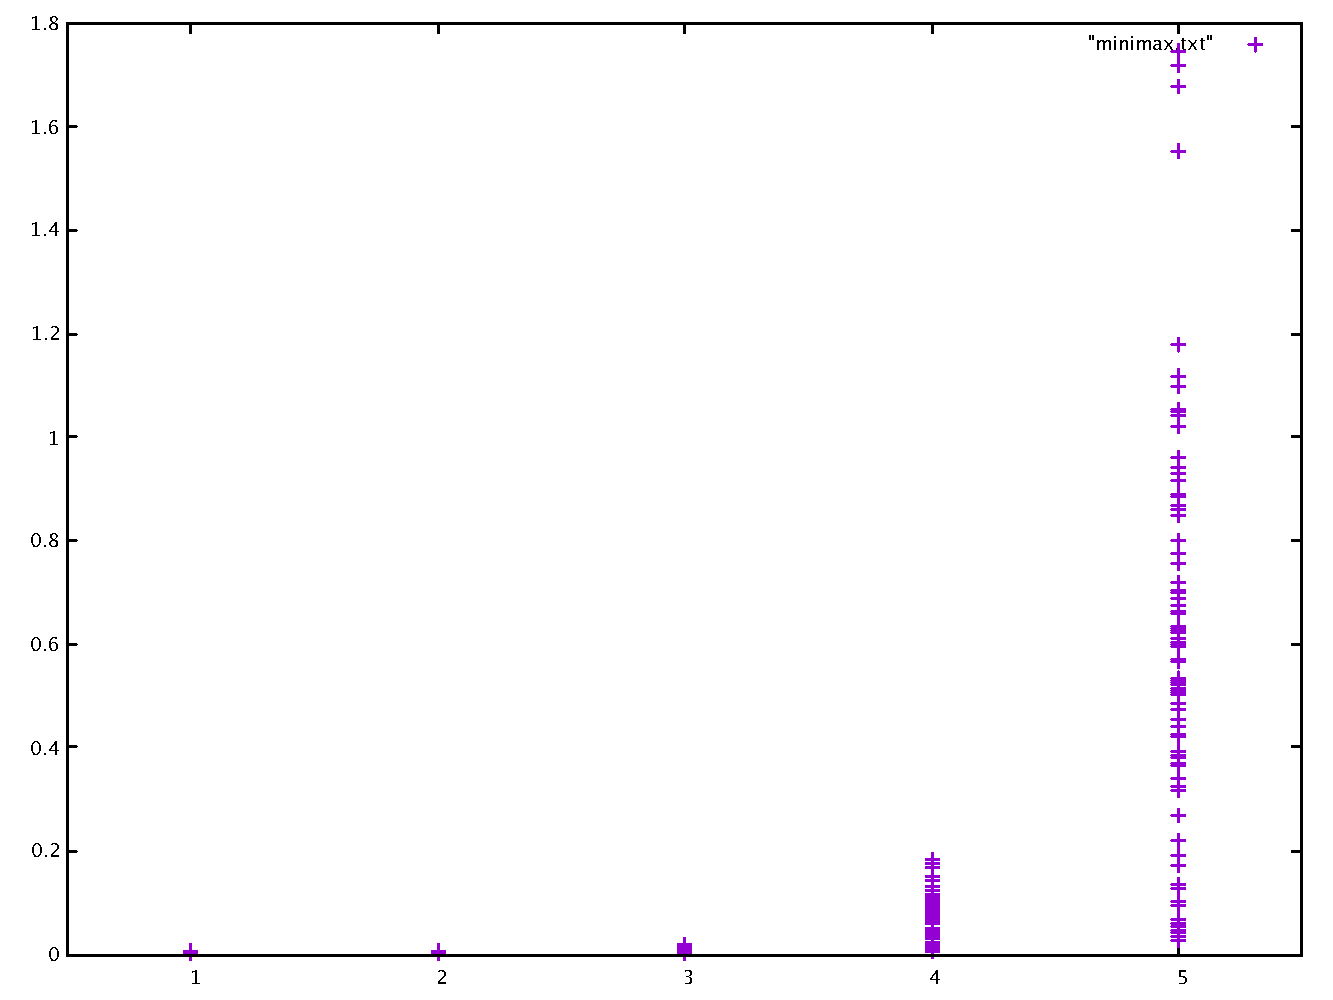
\includegraphics[width=10cm,keepaspectratio]{minimax.pdf}
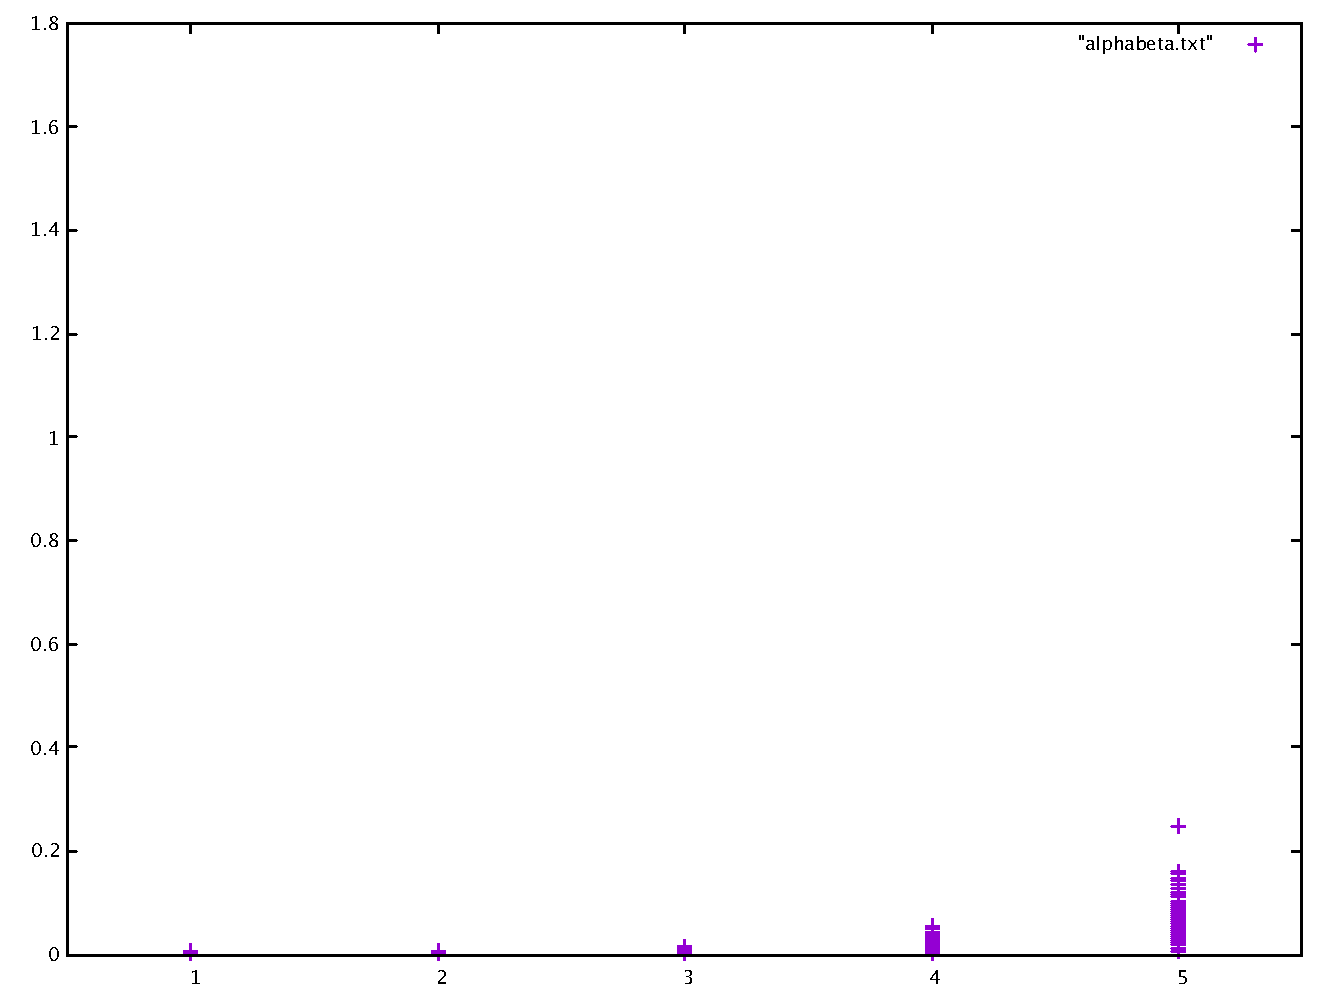
\includegraphics[width=10cm,keepaspectratio]{alphabeta.pdf}
\begin{center}
    \caption{Mini-Max \& Alpha-Beta}
\end{center}
\end{figure}

\end{document}
